
%=============== 2 sous-figures alignées horizontalement =================

\ifx \dispTwoFig \undefined
\def \dispTwoFig [#1]#2#3#4#5#6#7%
{
\begin{figure}[#1]
\begin{center}
  \subfloat[#3 \label{#7.a}]{\includegraphics[width=7cm, page=#2]{figs/figures}}\hspace{1cm}
  \subfloat[#5 \label{#7.b}]{\includegraphics[width=7cm, page=#4]{figs/figures}}\hspace{1cm}
  \caption{#6}  % legende \\
  \label{#7} % pour citer le numéro de figure
\end{center}
\end{figure}
}
\fi

%=============== 3 sous-figures alignées horizontalement =================

\ifx \dispThreeFig \undefined
\def \dispThreeFig [#1]#2#3#4#5#6#7#8#9%
{
\begin{figure}[#1]
\begin{center}
  \subfloat[#3 \label{#9.a}]{\includegraphics[width=5cm, page=#2]{figs/figures}}\hspace{1cm}
  \subfloat[#5 \label{#9.b}]{\includegraphics[width=5cm, page=#4]{figs/figures}}\hspace{1cm}
  \subfloat[#7 \label{#9.c}]{\includegraphics[width=5cm, page=#6]{figs/figures}}\\
  \caption{#8}  % legende
  \label{#9}    % pour citer le numéro de figure
\end{center}
\end{figure}
}
\fi

%=============== 2 ou 3 colonnes alignée horizontalement ==================

\ifx \minipages \undefined
\def \minipages [#1]#2#3#4#5#6#7%
{
\begin{minipage}{#2\textwidth}
  #5
\end{minipage}
\begin{minipage}{#3\textwidth} \hfill
  #6
\end{minipage}
\IfStrEq{#1}{3}%
{
\begin{minipage}{#4\textwidth} \hfill
  #7
\end{minipage}
}
}
\fi

%=============== Display 1 figure =========================================

\ifx \dispFig \undefined
\def \dispFig [#1]#2#3#4#5%
{
\begin{figure}[#1]
  \begin{center}
  \includegraphics[width=#3, page=#2]{figs/figures}
  \IfStrEq{#4}{}{}{%
    \caption{#4}  % legende
    \label{#5}    % pour citer le numéro de figure
  }
  \end{center}
\end{figure}
}
\fi

%=============== include 1 figure =========================================

\ifx \incFig \undefined
\def \incFig [#1]#2{\includegraphics[width=#2, page=#1]{figs/figures}}
\fi

%=============== exemples ==================================================

%\begin{minipage}{.3\textwidth} \hfill
%  \begin{align*}
%  D_{O} = \lbrace &\textbf{d}_{Ox}, \textbf{d}_{Oy}, \textbf{d}_{Oy}, \\
%  &\textbf{d}_{x}, \textbf{d}_{y}, \textbf{d}_{z} \rbrace \subset M^{6}
%  \end{align*}
%\end{minipage}
%\begin{minipage}{.4\textwidth} \hfill
%  \begin{tabbing}
%  \= $\textbf{d}_{Ox}$ \= vecteur unitaire de rotation autour de $O_{x}$\\
%  \> $\textbf{d}_{Oy}$ \> vecteur unitaire de rotation autour de $O_{y}$\\
%  \> $\textbf{d}_{Oz}$ \> vecteur unitaire de rotation autour de $O_{z}$\\
%  \> $\textbf{d}_{x}$  \> vecteur unitaire de translation le long de $O_{x}$\\
%  \> $\textbf{d}_{y}$  \> vecteur unitaire de translation le long de $O_{y}$\\
%  \> $\textbf{d}_{z}$  \> vecteur unitaire de translation le long de $O_{z}$\\
%  \end{tabbing}
%\end{minipage}

%=============== autres macro textuelles ===================================

\newcommand{\cad}[0]{c'est à dire }

